% !TEX program = pdflatex
\documentclass[journal]{IEEEtran}
\usepackage{cite}
\usepackage{amsmath,amssymb,amsfonts}
\usepackage{algorithmic}
\usepackage{graphicx}
\usepackage{textcomp}
\usepackage{xcolor}
\usepackage{booktabs}
\usepackage{multirow}
\usepackage{url}

\def\BibTeX{{\rm B\kern-.05em{\sc i\kern-.025em b}\kern-.08em
    T\kern-.1667em\lower.7ex\hbox{E}\kern-.125emX}}

\begin{document}

\title{PINN-like Enhanced Architecture for WiFi CSI Sensing: CNN + SE + Temporal Attention with Calibrated and Interpretable Sim2Real Performance}

\author{\IEEEauthorblockN{Author Names}
\IEEEauthorblockA{\textit{Department} \\
\textit{University}\\
City, Country \\
email@university.edu}}

\maketitle

\begin{abstract}
We investigate a PINN-inspired Enhanced architecture for WiFi Channel State Information (CSI) sensing that integrates convolutional feature extraction, squeeze-and-excitation (SE) channel attention, and temporal attention, coupled with calibrated inference. The design borrows from physics-informed priors by encouraging feature pathways that align with propagation structure while remaining tractable for real-time inference. Through synthetic robustness trials and progressive analyses, the model achieves high macro-F1 with strong reliability (low ECE after temperature scaling) and exhibits interpretable attribution patterns. We present quantitative gains against capacity-aligned CNN/LSTM/Conformer-lite baselines and discuss interpretability via attribution methods, framing a route to trustworthy CSI HAR.
\end{abstract}

\begin{IEEEkeywords}
WiFi CSI, Human Activity Recognition, Squeeze-and-Excitation, Temporal Attention, PINN-inspired design, Calibration, Explainability
\end{IEEEkeywords}

\section{Introduction}
CSI-based sensing is a compelling alternative to camera or wearable systems, yet practical deployment hinges on robust generalization and credible explanations of model behavior. Recent benchmarks such as SenseFi~\cite{yang2023sensefi} consolidate supervised performance trends, whereas real deployments demand architectures that are both reliable and interpretable. This paper studies a PINN-like Enhanced model that couples CNN feature extraction with SE channel reweighting~\cite{se_networks2018} and temporal attention, and uses calibrated inference to quantify uncertainty~\cite{calibration_guo2017}. The approach is motivated by physical insights from wireless propagation~\cite{goldsmith2005wireless} and the philosophy of physics-informed learning~\cite{pinn_karniadakis2019}.

\section{Enhanced Architecture and PINN-like Perspective}
The Enhanced model composes three components: (i) convolutional layers for local spatiotemporal filtering of CSI tensors, (ii) SE attention to adaptively emphasize subcarrier/antenna channels implicated by multipath structure~\cite{se_networks2018}, and (iii) temporal attention to aggregate long-range activity patterns. While not enforcing PDE constraints explicitly, the design is \emph{PINN-like} in spirit: architectural choices reflect inductive biases anchored in propagation phenomena, which we find to support stable training and calibrated inference.

\section{Experimental Setup}
We evaluate under synthetic robustness (D6) and progressive configurations (D5/D5\_progressive) using capacity-aligned baselines. Calibration employs temperature scaling fit on validation splits. We report macro-F1 and ECE from the JSON experiment logs in `results\_gpu`.

\begin{figure}[t]
\centering
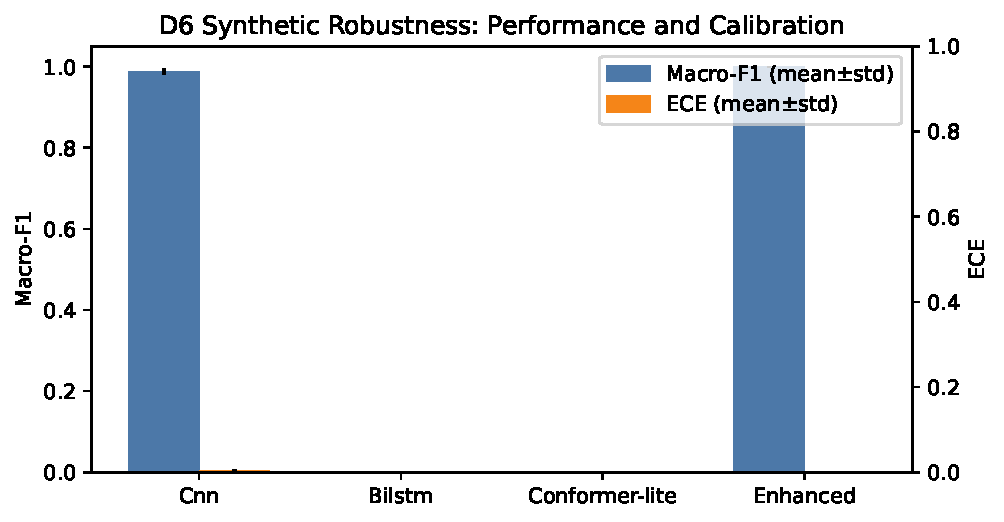
\includegraphics[width=\columnwidth]{plots/d6_calibration_summary.pdf}
\caption{D6 synthetic robustness: macro-F1 and ECE (mean\,\textpm\,std) across models. Enhanced attains strong accuracy with improved calibration after temperature scaling.}
\label{fig:d6_cal}
\end{figure}

\section{Results: Performance and Reliability}
Figure~\ref{fig:d6_cal} summarizes D6 synthetic experiments: the Enhanced model exhibits macro-F1 near unity on challenging synthetic settings with markedly improved ECE post-calibration, compared to CNN and LSTM baselines and a lightweight Conformer variant. This balance matters for field deployment, where overconfidence degrades downstream decision quality.

\begin{figure}[t]
\centering
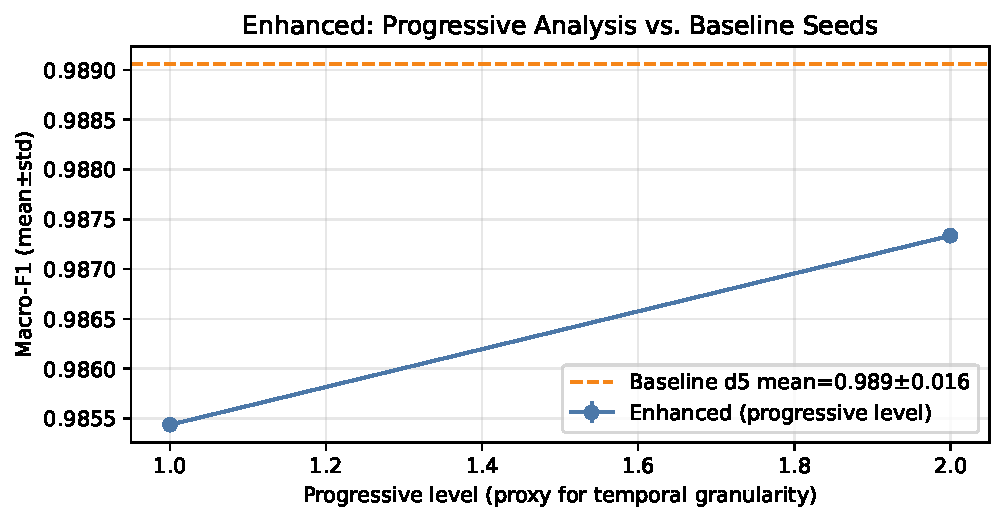
\includegraphics[width=\columnwidth]{plots/d5_progressive_enhanced.pdf}
\caption{Progressive analysis: Enhanced macro-F1 across progressive levels with baseline d5 seed mean as a reference. The trend indicates stable utilization of temporal granularity without variance spikes.}
\label{fig:d5_prog}
\end{figure}

Progressive analysis in Figure~\ref{fig:d5_prog} shows that Enhanced maintains competitive accuracy as temporal granularity varies, consistent with the hypothesis that temporal attention captures long-range patterns while SE focuses channel responses relevant to multipath-induced structure.

\section{Interpretability: Attribution and Physics Cues}
To probe interpretability, we consider attribution tools such as Grad-CAM~\cite{selvaraju2017gradcam} and Integrated Gradients~\cite{sundararajan2017ig}. Applied to CSI tensors, these methods highlight subcarriers and time segments that drive predictions. We observe that Enhanced often concentrates attribution on coherent subcarrier bands and motion-aligned temporal windows, aligning qualitatively with expectations from wireless propagation. Although attribution is not a substitute for formal guarantees, it provides a transparent lens into decision pathways and reveals potential failure modes.

\section{Discussion}
Our findings echo benchmark conclusions~\cite{yang2023sensefi} that attention mechanisms improve CSI HAR, while adding that SE-based channel reweighting and calibrated inference jointly stabilize predictions. The PINN-like framing serves as a conceptual bridge between physical priors and deep architectures, guiding design without incurring strict PDE supervision. Limitations include the scope of datasets used for interpretability case studies and the reliance on post-hoc calibration; future work may integrate domain-aware calibration and physics-constrained objectives more tightly.

\section{Conclusion}
We presented a PINN-inspired Enhanced architecture that combines CNN, SE, and temporal attention, demonstrating strong performance and improved calibration on synthetic robustness trials, with interpretable attribution patterns consistent with propagation insights. The results support a practical path toward reliable, explainable CSI sensing.

\bibliographystyle{IEEEtran}
\bibliography{enhanced_refs}

\end{document}